\chapter{Appendix}

\section{OPD vs Off-Policy Methods} \label{sec: exps_off_vs_on}

We compare the three distillation methods that only use feedback from the sampled token at each position. OPD uses the token sampled by the student and scores it under both the student and teacher policies. The two off-policy methods instead use teacher-generated rollouts: SFT treats the sampled token as a hard target, while the soft target objective also includes the teacher log probability for that sampled token.

The results in Figure~\ref{fig: opd_vs_off-policy} show that OPD is stronger than both off-policy methods across all evaluated student--teacher combinations. Among the off-policy methods, SFT consistently performs better than the soft target objective. The soft off-policy objective has worse absolute performance in every setting and also scales worse with teacher size: its gap recovery rate declines more sharply than SFT for both students. These results suggest that, when only the sampled token is available, adding the teacher's probability for a teacher-generated token is not enough to recover the benefit of training on the student's own rollout distribution.

\begin{figure}
    \centering
    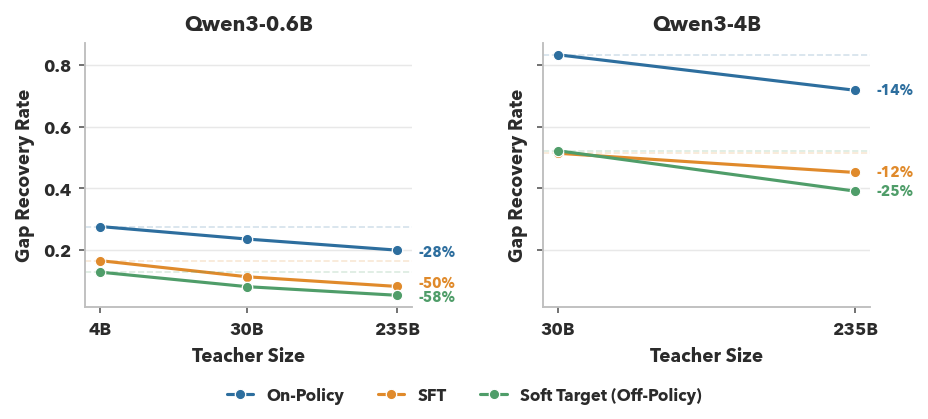
\includegraphics[width=0.9\linewidth]{figures/off_vs_on_policy.png}
    \caption{Gap recovery rate for the three distillation methods that use only the sampled token at each position. OPD performs best for both students across teacher sizes. Among the off-policy methods, SFT is consistently stronger than the soft target objective, which has lower gap recovery in every setting and degrades more when scaling the teacher.}
    \label{fig: opd_vs_off-policy}
\end{figure}

\FloatBarrier

\section{Catastrophic Forgetting in IFEval} \label{sec: app_ifeval_forgettin}

\begin{figure}
    \centering
    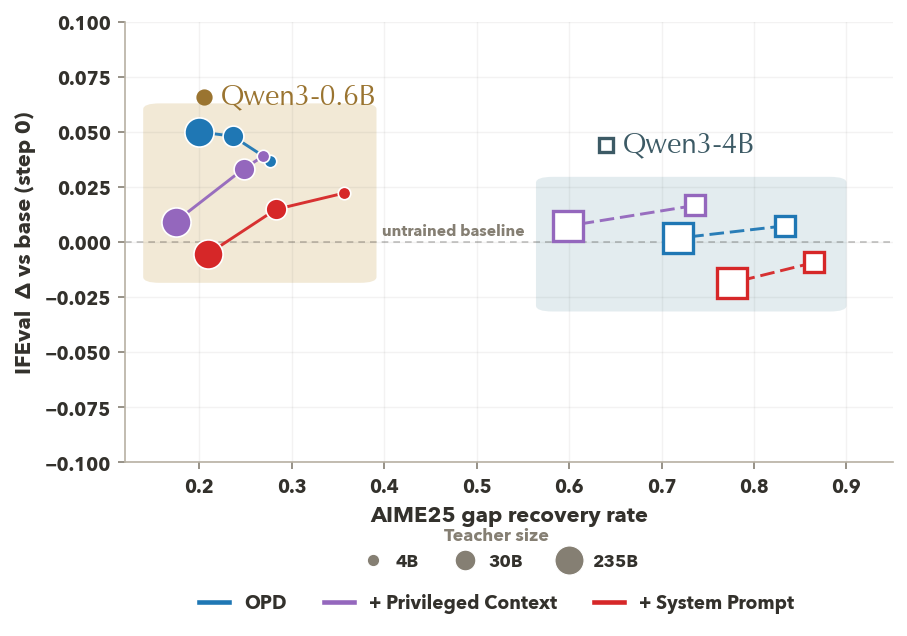
\includegraphics[width=0.9\linewidth]{figures/recovery_aime_vs_ifeval_delta.png}
    \caption{Caption}
    \label{fig: ifeval_reasoning}
\end{figure}

\FloatBarrier

\section{TAID Results}

\begin{figure}
    \centering
    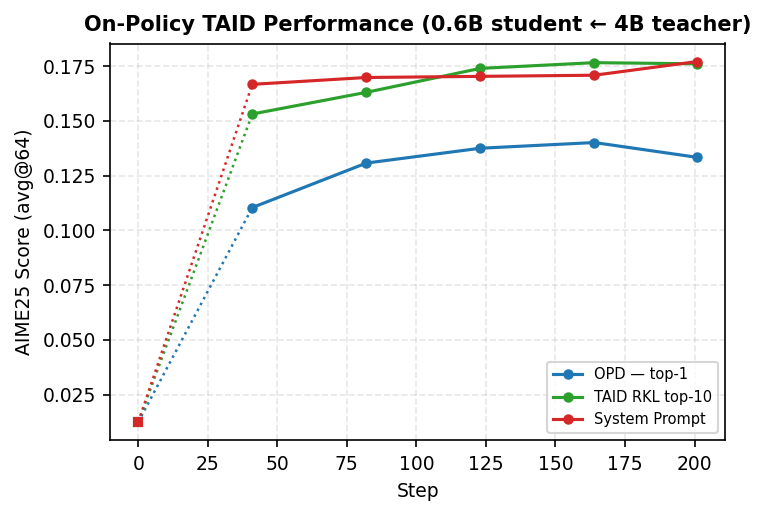
\includegraphics[width=0.9\linewidth]{figures/taid.png}
    \caption{Results for our on-policy implementation of TAID compared to OPD and with the system prompt setup from Section \ref{sec: exps_system_prompt}. The results show that TAID is a promising technique to address the capacity gap because its performance matches our best technique for the 0.6B student and 4B teacher combination.}
    \label{fig:placeholder}
\end{figure}

\FloatBarrier

\section{Hyperparameters} \label{app: hyperparameters}

\begin{table}[htbp]
    \centering
    \small
    \begin{tabular}{ll}
        \toprule
        Hyperparameter & Value \\
        \midrule
        \texttt{temperature} & \texttt{1.0} \\
        \texttt{lmbda} & \texttt{1.0} \\
        \texttt{beta} & \texttt{1.0} \\
        \texttt{max\_completion\_length} & \texttt{4096} \\
        \texttt{num\_generations} & \texttt{4} \\
        \texttt{use\_vllm} & \texttt{true} \\
        \texttt{vllm\_mode} & \texttt{colocate} \\
        \texttt{vllm\_gpu\_memory\_utilization} & \texttt{0.2} \\
        \texttt{bf16} & \texttt{true} \\
        \texttt{gradient\_accumulation\_steps} & \texttt{64} \\
        \texttt{max\_length} & \texttt{8192} \\
        \texttt{per\_device\_train\_batch\_size} & \texttt{1} \\
        \texttt{seed} & \texttt{42} \\
        \texttt{num\_train\_epochs} & \texttt{1} \\
        \texttt{learning\_rate} & \texttt{1e-6} \\
        \texttt{lr\_scheduler\_type} & \texttt{constant\_with\_warmup} \\
        \texttt{warmup\_steps} & \texttt{5} \\
        \bottomrule
    \end{tabular}
    \caption{General hyperparameters used for distillation training. The effective batch size if of 2048 given our 4 nodes with 8 GPUs each. For details on these hyperameters you can refer to \protect\url{https://huggingface.co/docs/trl/distillation_trainer\#trl.experimental.distillation.DistillationConfig}}
    \label{tab:distillation_hyperparameters}
\end{table}

\begin{table}[htbp]
    \centering
    \small
    \begin{tabular}{ll}
        \toprule
        Hyperparameter & Value \\
        \midrule
        \texttt{bf16} & \texttt{true} \\
        \texttt{gradient\_accumulation\_steps} & \texttt{2} \\
        \texttt{per\_device\_train\_batch\_size} & \texttt{4} \\
        \texttt{seed} & \texttt{42} \\
        \texttt{num\_train\_epochs} & \texttt{4} \\
        \texttt{use\_liger\_kernel} & \texttt{true} \\
        \texttt{packing} & \texttt{true} \\
        \texttt{max\_length} & \texttt{8192} \\
        \texttt{learning\_rate} & \texttt{5.0e-05} \\
        \texttt{lr\_scheduler\_type} & \texttt{cosine\_with\_min\_lr} \\
        \texttt{lr\_scheduler\_kwargs.min\_lr\_rate} & \texttt{0.1} \\
        \texttt{warmup\_ratio} & \texttt{0.05} \\
        \bottomrule
    \end{tabular}
    \caption{Hyperparameters used for SFT training. The effective batch size if of 128 given our 4 nodes with 8 GPUs each. For details on these hyperameters you can refer to \protect\url{https://huggingface.co/docs/trl/sft_trainer\#trl.sft.SFTConfig}}
    \label{tab:sft_hyperparameters}
\end{table}

\FloatBarrier

\section{Privileged Information Prompts} \label{app: pc_prompts}

\begin{figure}
    \centering
\begin{tcblisting}{
    enhanced,
    listing only,
    title={Larger-Teacher Rollout Privileged Context},
    fonttitle=\bfseries,
    coltitle=white,
    colback=green!2,
    colframe=green!45!black,
    boxrule=0.6pt,
    arc=1.5mm,
    left=2mm,
    right=2mm,
    top=1.5mm,
    bottom=1.5mm,
    listing options={
        basicstyle=\ttfamily\scriptsize,
        breaklines=true,
        columns=fullflexible,
        keepspaces=true,
        showstringspaces=false,
        escapeinside={(*@}{@*)}
    }
}
(*@\textcolor{blue!70!black}{\texttt{\{prompt\}}}@*)

This is an example for a response to the question:

(*@\textcolor{blue!70!black}{\texttt{\{larger\_teacher\_rollout\}}}@*)
\end{tcblisting}
    \caption{Prompt template used to provide the intermediate teacher with a larger teacher's rollout as privileged context. The student does not see this context when generating its own rollout. The \texttt{prompt} placeholder contains the problem description and the \texttt{larger\_teacher\_rollout} is replaced by the teacher rollout for the prompt.}
    \label{fig: pc_rollout_example}
\end{figure}
